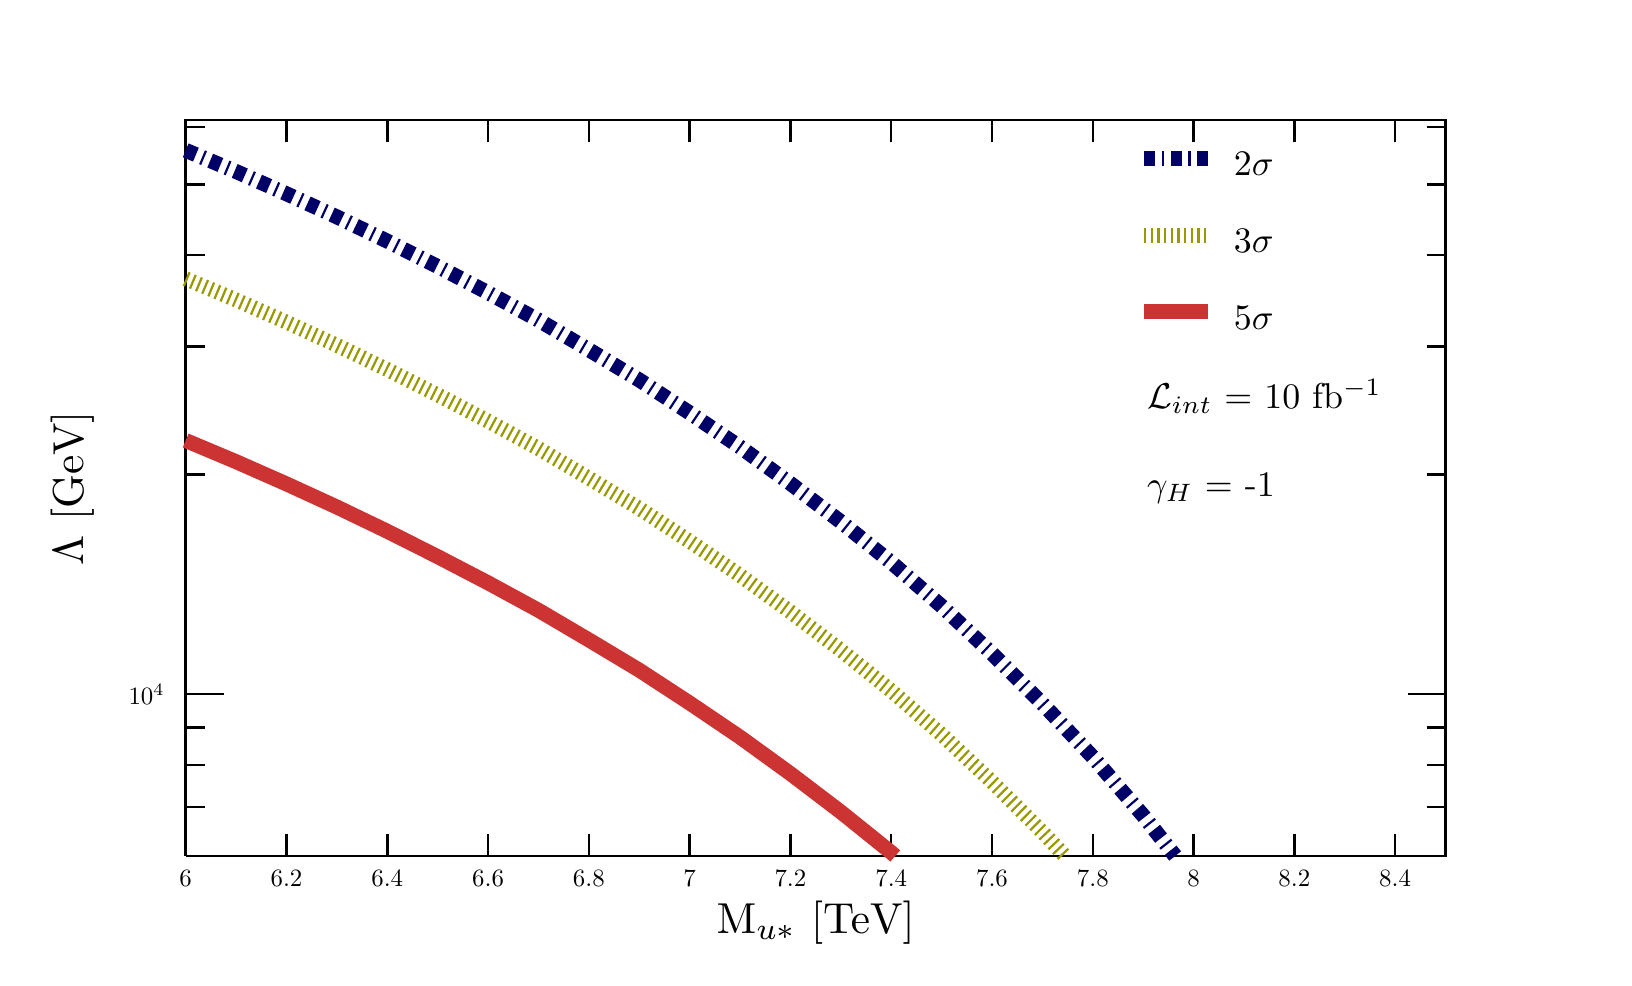
\begin{tikzpicture}
\pgfdeclareplotmark{cross} {
\pgfpathmoveto{\pgfpoint{-0.3\pgfplotmarksize}{\pgfplotmarksize}}
\pgfpathlineto{\pgfpoint{+0.3\pgfplotmarksize}{\pgfplotmarksize}}
\pgfpathlineto{\pgfpoint{+0.3\pgfplotmarksize}{0.3\pgfplotmarksize}}
\pgfpathlineto{\pgfpoint{+1\pgfplotmarksize}{0.3\pgfplotmarksize}}
\pgfpathlineto{\pgfpoint{+1\pgfplotmarksize}{-0.3\pgfplotmarksize}}
\pgfpathlineto{\pgfpoint{+0.3\pgfplotmarksize}{-0.3\pgfplotmarksize}}
\pgfpathlineto{\pgfpoint{+0.3\pgfplotmarksize}{-1.\pgfplotmarksize}}
\pgfpathlineto{\pgfpoint{-0.3\pgfplotmarksize}{-1.\pgfplotmarksize}}
\pgfpathlineto{\pgfpoint{-0.3\pgfplotmarksize}{-0.3\pgfplotmarksize}}
\pgfpathlineto{\pgfpoint{-1.\pgfplotmarksize}{-0.3\pgfplotmarksize}}
\pgfpathlineto{\pgfpoint{-1.\pgfplotmarksize}{0.3\pgfplotmarksize}}
\pgfpathlineto{\pgfpoint{-0.3\pgfplotmarksize}{0.3\pgfplotmarksize}}
\pgfpathclose
\pgfusepathqstroke
}
\pgfdeclareplotmark{cross*} {
\pgfpathmoveto{\pgfpoint{-0.3\pgfplotmarksize}{\pgfplotmarksize}}
\pgfpathlineto{\pgfpoint{+0.3\pgfplotmarksize}{\pgfplotmarksize}}
\pgfpathlineto{\pgfpoint{+0.3\pgfplotmarksize}{0.3\pgfplotmarksize}}
\pgfpathlineto{\pgfpoint{+1\pgfplotmarksize}{0.3\pgfplotmarksize}}
\pgfpathlineto{\pgfpoint{+1\pgfplotmarksize}{-0.3\pgfplotmarksize}}
\pgfpathlineto{\pgfpoint{+0.3\pgfplotmarksize}{-0.3\pgfplotmarksize}}
\pgfpathlineto{\pgfpoint{+0.3\pgfplotmarksize}{-1.\pgfplotmarksize}}
\pgfpathlineto{\pgfpoint{-0.3\pgfplotmarksize}{-1.\pgfplotmarksize}}
\pgfpathlineto{\pgfpoint{-0.3\pgfplotmarksize}{-0.3\pgfplotmarksize}}
\pgfpathlineto{\pgfpoint{-1.\pgfplotmarksize}{-0.3\pgfplotmarksize}}
\pgfpathlineto{\pgfpoint{-1.\pgfplotmarksize}{0.3\pgfplotmarksize}}
\pgfpathlineto{\pgfpoint{-0.3\pgfplotmarksize}{0.3\pgfplotmarksize}}
\pgfpathclose
\pgfusepathqfillstroke
}
\pgfdeclareplotmark{newstar} {
\pgfpathmoveto{\pgfqpoint{0pt}{\pgfplotmarksize}}
\pgfpathlineto{\pgfqpointpolar{44}{0.5\pgfplotmarksize}}
\pgfpathlineto{\pgfqpointpolar{18}{\pgfplotmarksize}}
\pgfpathlineto{\pgfqpointpolar{-20}{0.5\pgfplotmarksize}}
\pgfpathlineto{\pgfqpointpolar{-54}{\pgfplotmarksize}}
\pgfpathlineto{\pgfqpointpolar{-90}{0.5\pgfplotmarksize}}
\pgfpathlineto{\pgfqpointpolar{234}{\pgfplotmarksize}}
\pgfpathlineto{\pgfqpointpolar{198}{0.5\pgfplotmarksize}}
\pgfpathlineto{\pgfqpointpolar{162}{\pgfplotmarksize}}
\pgfpathlineto{\pgfqpointpolar{134}{0.5\pgfplotmarksize}}
\pgfpathclose
\pgfusepathqstroke
}
\pgfdeclareplotmark{newstar*} {
\pgfpathmoveto{\pgfqpoint{0pt}{\pgfplotmarksize}}
\pgfpathlineto{\pgfqpointpolar{44}{0.5\pgfplotmarksize}}
\pgfpathlineto{\pgfqpointpolar{18}{\pgfplotmarksize}}
\pgfpathlineto{\pgfqpointpolar{-20}{0.5\pgfplotmarksize}}
\pgfpathlineto{\pgfqpointpolar{-54}{\pgfplotmarksize}}
\pgfpathlineto{\pgfqpointpolar{-90}{0.5\pgfplotmarksize}}
\pgfpathlineto{\pgfqpointpolar{234}{\pgfplotmarksize}}
\pgfpathlineto{\pgfqpointpolar{198}{0.5\pgfplotmarksize}}
\pgfpathlineto{\pgfqpointpolar{162}{\pgfplotmarksize}}
\pgfpathlineto{\pgfqpointpolar{134}{0.5\pgfplotmarksize}}
\pgfpathclose
\pgfusepathqfillstroke
}
\definecolor{c}{rgb}{1,1,1};
\draw [color=c, fill=c] (0,0) rectangle (20,11.6806);
\draw [color=c, fill=c] (2,1.16806) rectangle (18,10.5125);
\definecolor{c}{rgb}{0,0,0};
\draw [c,line width=0.9] (2,1.16806) -- (2,10.5125) -- (18,10.5125) -- (18,1.16806) -- (2,1.16806);
\definecolor{c}{rgb}{1,1,1};
\draw [color=c, fill=c] (2,1.16806) rectangle (18,10.5125);
\definecolor{c}{rgb}{0,0,0};
\draw [c,line width=0.9] (2,1.16806) -- (2,10.5125) -- (18,10.5125) -- (18,1.16806) -- (2,1.16806);
\draw [c,line width=0.9] (2,1.16806) -- (18,1.16806);
\draw (10,0.327056) node[scale=1.56475, color=c, rotate=0]{M$_{u*}$ [TeV]};
\draw [c,line width=0.9] (2,1.44839) -- (2,1.16806);
\draw [c,line width=0.9] (3.28,1.44839) -- (3.28,1.16806);
\draw [c,line width=0.9] (4.56,1.44839) -- (4.56,1.16806);
\draw [c,line width=0.9] (5.84,1.44839) -- (5.84,1.16806);
\draw [c,line width=0.9] (7.12,1.44839) -- (7.12,1.16806);
\draw [c,line width=0.9] (8.4,1.44839) -- (8.4,1.16806);
\draw [c,line width=0.9] (9.68,1.44839) -- (9.68,1.16806);
\draw [c,line width=0.9] (10.96,1.44839) -- (10.96,1.16806);
\draw [c,line width=0.9] (12.24,1.44839) -- (12.24,1.16806);
\draw [c,line width=0.9] (13.52,1.44839) -- (13.52,1.16806);
\draw [c,line width=0.9] (14.8,1.44839) -- (14.8,1.16806);
\draw [c,line width=0.9] (16.08,1.44839) -- (16.08,1.16806);
\draw [c,line width=0.9] (17.36,1.44839) -- (17.36,1.16806);
\draw [c,line width=0.9] (17.36,1.44839) -- (17.36,1.16806);
\draw [anchor=base] (2,0.782598) node[scale=0.900036, color=c, rotate=0]{6};
\draw [anchor=base] (3.28,0.782598) node[scale=0.900036, color=c, rotate=0]{6.2};
\draw [anchor=base] (4.56,0.782598) node[scale=0.900036, color=c, rotate=0]{6.4};
\draw [anchor=base] (5.84,0.782598) node[scale=0.900036, color=c, rotate=0]{6.6};
\draw [anchor=base] (7.12,0.782598) node[scale=0.900036, color=c, rotate=0]{6.8};
\draw [anchor=base] (8.4,0.782598) node[scale=0.900036, color=c, rotate=0]{7};
\draw [anchor=base] (9.68,0.782598) node[scale=0.900036, color=c, rotate=0]{7.2};
\draw [anchor=base] (10.96,0.782598) node[scale=0.900036, color=c, rotate=0]{7.4};
\draw [anchor=base] (12.24,0.782598) node[scale=0.900036, color=c, rotate=0]{7.6};
\draw [anchor=base] (13.52,0.782598) node[scale=0.900036, color=c, rotate=0]{7.8};
\draw [anchor=base] (14.8,0.782598) node[scale=0.900036, color=c, rotate=0]{8};
\draw [anchor=base] (16.08,0.782598) node[scale=0.900036, color=c, rotate=0]{8.2};
\draw [anchor=base] (17.36,0.782598) node[scale=0.900036, color=c, rotate=0]{8.4};
\draw [c,line width=0.9] (2,10.5125) -- (18,10.5125);
\draw [c,line width=0.9] (2,10.2322) -- (2,10.5125);
\draw [c,line width=0.9] (3.28,10.2322) -- (3.28,10.5125);
\draw [c,line width=0.9] (4.56,10.2322) -- (4.56,10.5125);
\draw [c,line width=0.9] (5.84,10.2322) -- (5.84,10.5125);
\draw [c,line width=0.9] (7.12,10.2322) -- (7.12,10.5125);
\draw [c,line width=0.9] (8.4,10.2322) -- (8.4,10.5125);
\draw [c,line width=0.9] (9.68,10.2322) -- (9.68,10.5125);
\draw [c,line width=0.9] (10.96,10.2322) -- (10.96,10.5125);
\draw [c,line width=0.9] (12.24,10.2322) -- (12.24,10.5125);
\draw [c,line width=0.9] (13.52,10.2322) -- (13.52,10.5125);
\draw [c,line width=0.9] (14.8,10.2322) -- (14.8,10.5125);
\draw [c,line width=0.9] (16.08,10.2322) -- (16.08,10.5125);
\draw [c,line width=0.9] (17.36,10.2322) -- (17.36,10.5125);
\draw [c,line width=0.9] (17.36,10.2322) -- (17.36,10.5125);
\draw [c,line width=0.9] (2,1.16806) -- (2,10.5125);
\draw (0.56,5.84029) node[scale=1.56475, color=c, rotate=90]{$\Lambda$ [GeV]};
\draw [c,line width=0.9] (2.24,1.16872) -- (2,1.16872);
\draw [c,line width=0.9] (2.24,1.78865) -- (2,1.78865);
\draw [c,line width=0.9] (2.24,2.32566) -- (2,2.32566);
\draw [c,line width=0.9] (2.24,2.79933) -- (2,2.79933);
\draw [c,line width=0.9] (2.48,3.22305) -- (2,3.22305);
\draw [anchor= east] (1.844,3.22305) node[scale=0.900036, color=c, rotate=0]{$10^{4}$};
\draw [c,line width=0.9] (2.24,6.0106) -- (2,6.0106);
\draw [c,line width=0.9] (2.24,7.64121) -- (2,7.64121);
\draw [c,line width=0.9] (2.24,8.79815) -- (2,8.79815);
\draw [c,line width=0.9] (2.24,9.69554) -- (2,9.69554);
\draw [c,line width=0.9] (2.24,10.4288) -- (2,10.4288);
\draw [c,line width=0.9] (18,1.16806) -- (18,10.5125);
\draw [c,line width=0.9] (17.76,1.16872) -- (18,1.16872);
\draw [c,line width=0.9] (17.76,1.78865) -- (18,1.78865);
\draw [c,line width=0.9] (17.76,2.32566) -- (18,2.32566);
\draw [c,line width=0.9] (17.76,2.79933) -- (18,2.79933);
\draw [c,line width=0.9] (17.52,3.22305) -- (18,3.22305);
\draw [c,line width=0.9] (17.76,6.0106) -- (18,6.0106);
\draw [c,line width=0.9] (17.76,7.64121) -- (18,7.64121);
\draw [c,line width=0.9] (17.76,8.79815) -- (18,8.79815);
\draw [c,line width=0.9] (17.76,9.69554) -- (18,9.69554);
\draw [c,line width=0.9] (17.76,10.4288) -- (18,10.4288);
\definecolor{c}{rgb}{0,0,0.4};
\draw [c,dash pattern=on 4.00pt off 2.40pt on 0.80pt off 2.40pt ,line width=5.4] (2,10.1295) -- (2.64,9.86039) -- (3.28,9.57798) -- (3.92,9.28458) -- (4.56,8.97656) -- (5.2,8.65455) -- (5.84,8.32155) -- (6.48,7.97342) -- (7.12,7.59685) --
 (7.76,7.21285) -- (8.4,6.79522) -- (9.04,6.36239) -- (9.68,5.89881) -- (10.32,5.41225) -- (10.96,4.89737) -- (11.6,4.34107) -- (12.24,3.73894) -- (12.88,3.10311) -- (13.52,2.42463) -- (14.16,1.68117) -- (14.566,1.16806);
\definecolor{c}{rgb}{0.6,0.6,0};
\draw [c,dash pattern=on 0.80pt off 1.60pt ,line width=5.4] (2,8.49885) -- (2.64,8.22978) -- (3.28,7.94737) -- (3.92,7.65397) -- (4.56,7.34595) -- (5.2,7.02394) -- (5.84,6.69095) -- (6.48,6.3428) -- (7.12,5.96624) -- (7.76,5.58224) -- (8.4,5.16461)
 -- (9.04,4.73178) -- (9.68,4.2682) -- (10.32,3.78166) -- (10.96,3.26673) -- (11.6,2.71044) -- (12.24,2.10833) -- (12.88,1.4725) -- (13.1672,1.16806);
\definecolor{c}{rgb}{0.8,0.2,0.2};
\draw [c,line width=5.4] (2,6.44451) -- (2.64,6.17544) -- (3.28,5.89304) -- (3.92,5.59965) -- (4.56,5.29163) -- (5.2,4.96962) -- (5.84,4.63662) -- (6.48,4.28846) -- (7.12,3.91193) -- (7.76,3.5279) -- (8.4,3.11029) -- (9.04,2.67746) -- (9.68,2.21388)
 -- (10.32,1.72732) -- (10.96,1.21243) -- (11.011,1.16806);
\definecolor{c}{rgb}{0,0,0};
\draw (10,11.301) node[scale=1.2177, color=c, rotate=0]{ };
\draw [anchor=base west] (15.15,9.80681) node[scale=1.29711, color=c, rotate=0]{$2\sigma$};
\definecolor{c}{rgb}{0,0,0.4};
\draw [c,dash pattern=on 4.00pt off 2.40pt on 0.80pt off 2.40pt ,line width=5.4] (14.1725,10.0258) -- (14.9775,10.0258);
\definecolor{c}{rgb}{0,0,0};
\draw [anchor=base west] (15.15,8.83343) node[scale=1.29711, color=c, rotate=0]{$3\sigma$};
\definecolor{c}{rgb}{0.6,0.6,0};
\draw [c,dash pattern=on 0.80pt off 1.60pt ,line width=5.4] (14.1725,9.05244) -- (14.9775,9.05244);
\definecolor{c}{rgb}{0,0,0};
\draw [anchor=base west] (15.15,7.86005) node[scale=1.29711, color=c, rotate=0]{$5\sigma$};
\definecolor{c}{rgb}{0.8,0.2,0.2};
\draw [c,line width=5.4] (14.1725,8.07906) -- (14.9775,8.07906);
\definecolor{c}{rgb}{0,0,0};
\draw [anchor= west] (14.05,7.00834) node[scale=1.29711, color=c, rotate=0]{$\mathcal{L}_{int}$ = 10 fb$^{-1}$};
\draw [anchor= west] (14.05,5.84029) node[scale=1.29711, color=c, rotate=0]{$\gamma_{H}$ = -1};
\end{tikzpicture}
